深層学習は2012年のImageNetチャレンジ\cite{ILSVRC15}でAlexNet\cite{krizhevsky2012imagenet}が大きな成功を収めて以来,急速に発展し,あらゆるタスクにおいて高度な能力を発揮している\cite{alom2018history}.
これは画像処理の分野では特に顕著で,医療画像処理も例外ではない\cite{litjens2017survey}.
しかし,深層学習に関する基礎的な考え方が成立したのは1940年代である\cite{Goodfellow-et-al-2016}.
そして,現在多く研究されているような畳み込みニューラルネットワーク(Convolutional Neural Network;CNN)\cite{lecun1998gradient}の基礎となっているネオコグニトロン\cite{fukushima1982neocognitron}が発表されたのは1982年であり,今日の深層学習技術を理解するにはそれらの簡単な歴史的経緯および理論的背景を学ぶことが重要である.

本節では前節で触れた機械学習の基礎となる線形回帰およびロジスティック回帰と深層学習の関連に触れつつ,深層学習の基礎的な考えを示す.

\subsection{多層パーセプトロン}
    人工ニューラルネットワーク(Artificial Neural Network;ANN)は生物学的学習の計算機モデルであり,脳の中で学習が行われている様子を模倣して,計算機のためのモデルに落とし込んだものである.
    パーセプトロンは最も単純なニューラルネットワークモデルであり,複数の信号を受け取り,一つの信号を出力するアルゴリズムである.
    出力されるのは信号を流す(1)か流さない(0)かの2値である.
    パーセプトロンは以下の数式\ref{neuron}で表される.
    ここで入力は$x$, 出力は$y$で表され, $\theta$は閾値とする.

    \begin{eqnarray}
        a&=&\sum_{j}w_{j}x_{j}+b \nonumber \\
        y&=&\left
                \{
                \begin{array}{ll}
                1 & (a\geq \theta) \\
                0 & (a<\theta) \\
                \end{array}
            \right.
        \label{neuron}
    \end{eqnarray}
    パーセプトロンの概要図を\ref{perceptron}に示した.
    \begin{figure}[ht]
      \centering
      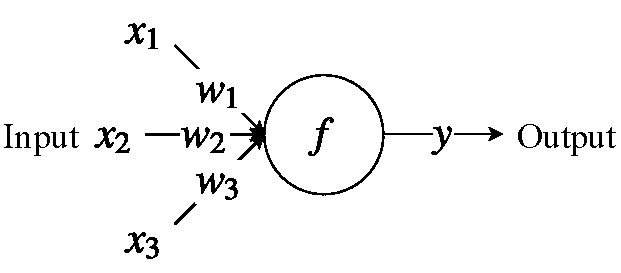
\includegraphics[width=10cm]{8_appendix/img/perceptron.pdf}
      \caption{Perceptron.}
      \label{perceptron}
    \end{figure}
    ここで,閾値(threshold)は,人工ニューロンにおける重み$w_{i}$と同様に学習によって変化するパラメータの一種であり,左辺に移し,バイアス$b$として置き換えると,次のようになる.
    \begin{align}
      y =   \begin{cases}
                0 \quad\text{if}\quad \sum_{j}w_{j}x_{j} + b \leq 0 \\
                1 \quad\text{if}\quad \sum_{j}w_{j}x_{j} + b > 0
            \end{cases}
    \end{align}
    このように,人工ニューロンの働きは,入力$x$に応じて値を出力する関数$f$として考えることができる.
    ここで,このパーセプトロンが前節における一般化線形モデルと同等であることに注意されたい.

    以上のようにパーセプトロンは線形分類器として利用ができる.
    つまり以下の図\ref{gate}中(a)(b)のように論理回路のAND素子やOR素子を実装することができる.
    パーセプトロンの出力部分を上記の式ではしきい値によって制御したが, この部分は一般化線形モデルにおける活性化関数を用いて実装できる.
    つまり,この場合には活性化関数としてステップ関数が用いられていると言える.
    通常,この活性化関数にはシグモイド関数やtanhなどの微分可能な関数が用いられる.
    微分可能な関数が用いられる理由については,後述の誤差逆伝播法を参照されたい.
    以下に,ニューラルネットワークに用いられる主な活性化関数を列挙する.
    
    \begin{itemize}
        \item 恒等写像関数
            \begin{equation}
                h(x)=x
            \end{equation}
        \item ステップ関数
            \begin{align}
              h(x)= \begin{cases}
                        1 \quad\text{if}\quad x \geq 0 \\
                        0 \quad\text{if}\quad x < 0
                    \end{cases}
            \end{align}
        \item sigmoid関数
            \begin{equation}
                h(x)=\frac{1}{1+e^{-\bm{w}^T\bm{x}}}
            \end{equation}
        \item tanh関数
            \begin{equation}
                h(x)=tanh(x)=\frac{\sinh(x)}{\cosh(x)}=\frac{e^x-e^{-x}}{e^x+e^{-x}}
            \end{equation}
        \item Rectified Linear Unit (ReLU)関数\cite{nair2010rectified}
            \begin{align}
              h(x)= \begin{cases}
                        x \quad\text{if}\quad x \geq 0 \\
                        0 \quad\text{if}\quad x < 0
                    \end{cases}
            \end{align}
        \item LeakyReLU関数\cite{maas2013rectifier}
            \begin{align}
              h(x)= \begin{cases}
                        x \quad\text{if}\quad x \geq 0 \\
                        ax \quad\text{if}\quad x < 0
                    \end{cases}
            \end{align}
        \item Softplus関数\cite{dugas2001incorporating}
            \begin{equation}
                h(x)=\log{(1+\exp(x))}
            \end{equation}
        \item Hardtanh関数
            \begin{align}
              h(x)= \begin{cases}
                        x \quad\text{if}\quad -1 \leq x \geq 1 \\
                        1 \quad\text{if}\quad x > 1 \\
                        -1 \quad\text{if}\quad x < -1
                    \end{cases}
            \end{align}
        \item Softmax関数
            \begin{equation}
                y_k = \frac{\exp{a_k}}{\sum^K_{i=1}\exp{\left(a_i\right)}}
            \end{equation}
    \end{itemize}

    さらにパーセプトロンを多層に重ねたものを多層パーセプトロンと呼び, NAND素子については図\ref{gate}中(c)のように3層パーセプトロンで実装できる.
    以上のように多層パーセプトロンは非線形な分類問題にも対応している.
    
    \begin{figure}[ht]
        \begin{center}
            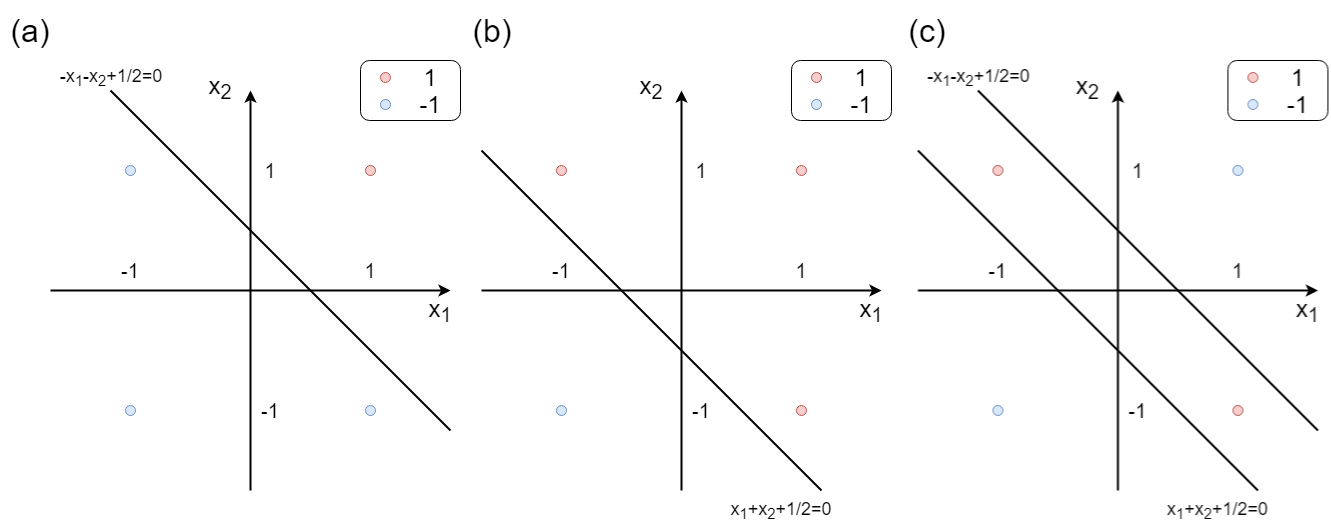
\includegraphics[width=16.0cm]{./8_appendix/img/gate.png}
            \caption{logic circuits implemented by formal neurons (a) AND gate (b)OR gate (c) NANDgate using a three-layer perceptron.}
            \label{gate}
        \end{center}
    \end{figure}
    
    この多層パーセプトロンを基礎とする人工ニューラルネットワークは,単純にニューラルネットワークと呼ばれることが多い.
    ニューラルネットワークにおいて,値の入力をする層を入力層,出力をする層を出力層という.
    そして,これら入力層と出力層の間に存在する多数の中間層を隠れ層という.
    図\ref{fig:mlperceptron}のようなニューラルネットワークでは,入力層から入力されたデータが中間層を経て出力層へと順番に計算,伝播していくため,順伝播型ニューラルネットワークと呼ばれる.

    \begin{figure}[ht]
        \begin{center}
            \centering
            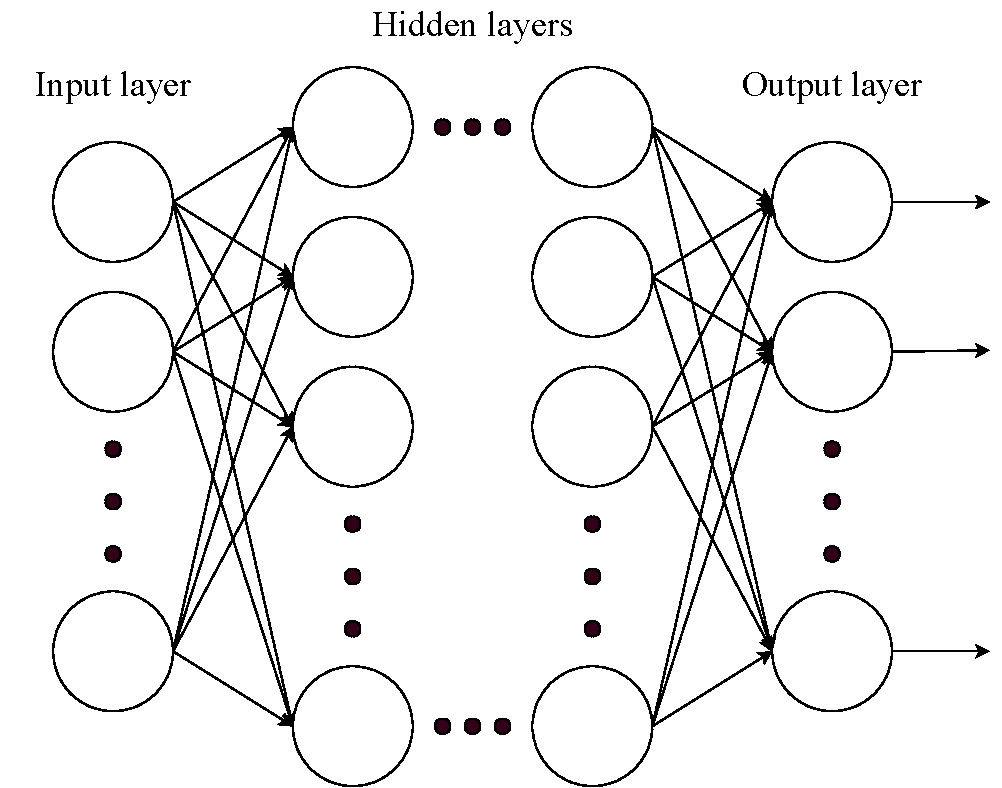
\includegraphics[width=10cm]{8_appendix/img/multi_layer_perceptron.pdf}
            \caption{Multi layer perceptron.}
            \label{fig:mlperceptron}
        \end{center}
    \end{figure}
    パーセプトロンの多層化により,様々な入力$x$と出力$y$の関係を同時に表すことができるようになった.
    例えば,Hornikら\cite{hornik1989multilayer}やCybenko\cite{cybenko1989approximation}らの万能近似定理(universal approximation theorem)によると,ネットワークが十分な数の隠れユニットを持つ場合,線形の出力層とシグモイド関数のような「押しつぶす」活性化関数をもつ隠れ層が少なくとも1つ含まれる順伝播型ネットワークは,どんなボレル可測関数でも任意の精度で近似できると述べられている.
    つまり,ノードを増やしていくと,ニューラルネットワークの表現力は上昇していき,学習データをほぼ完全に説明できるニューラルネットワークが実現できる.
    ただし,学習データを完全に説明できるモデルが実現した場合でも,そのモデルの汎化性能が必ずしも高いわけではないことに注意されたい.

\subsection{勾配に基づく最適化}
    このニューラルネットワークは,今まで示した通り,非常に高度な表現力を有する.
    しかし,このモデルのパラメータは線形回帰やロジスティック回帰のように解析的に求めることはできない.
    ニューラルネットワークの学習では,線形回帰やロジスティック回帰と同様に,モデルの指標として損失関数が定義され,損失関数を最小化することによって学習が行われる.
    ニューラルネットワークの場合,この損失関数の解空間が度重なる非線形変換によって非常に複雑になる(非凸となる).
    また,膨大な量のデータを学習することが多いため,一度にすべてのデータに対して計算が実行不可能であることなども問題である.
    
    そこでニューラルネットワークの訓練には,最急降下法\cite{cauchy1847methode}(または勾配降下法)がよく用いられる.
    この手法の発想は非常に単純である.
    最急降下法は,ある関数の一点に関して勾配(微分)を計算することにより,最も勾配が急である方向に向けてパラメータを動かす手法である.
    ここで,非常に単純化した最急降下法を用いたパラメータの更新式を以下に示す.
    \begin{equation}
        w^{(i+1)}=w^{(i)}-\eta\frac{\partial f_w}{\partial w^{(i)}}
    \end{equation}
    ここで$\eta$は学習率と呼ばれる,学習速度を調整するためのハイパーパラメータである.
    
    以上の単純な式を念頭におき,実際にどのように最急降下法が動作するかを詳しく見ていく.
    ニューラルネットワークに入力$\bm{x}^{\text{T}} = (x_{1}, x_{2}, x_{3})$を入力したときの出力が$\bm{y}^{\text{T}} = (y_{1}, y_{2})$であったとする.
    このとき目標とする出力を$\bm{t}^{\text{T}} = (t_{1}, t_{2})$とし,その誤差を$E(\bm{y}, \bm{t})$とする.このとき,ニューラルネットワークは誤差$E$を最小化する$\hat{\bm{y}}$を出力することを目的とし,学習が行われる.この条件は以下の式で表される.
    \begin{equation}
      \hat{\bm{y}} = \rm{argmin}_{\bm{y}}(E(\bm{y}, \bm{t}))
    \end{equation}
    ここで,$\hat{\bm{y}}$を解析的に求めることは困難であることは先程述べた.そこで,
    $\bm{y}$を微小量$\delta\bm{y}$だけ変化させた際の誤差$E(\bm{y}+\delta \bm{y}, \bm{t})$が$E(\bm{y}, \bm{t})$よりも小さくなる状態を考える.つまり,
    \begin{align}
      E (\bm{y} + \delta \bm{y}, \bm{t}) < E(\bm{y}, \bm{t}) 
      \label{eq:e_hikaku}
    \end{align}
    を満たすような$\delta\bm{y}$を求める.ここで,$E(\bm{y}+\delta \bm{y}, \bm{t})$はテイラー展開により次のように近似される.
    \begin{align}
      E(\bm{y}+\delta\bm{y}, t) &\approx E(\bm{y}, \bm{t}) + \frac{\partial E(\bm{y}, \bm{t})}{\partial \bm{y}} \delta \bm{y}
      \label{eq:e_taylor}
    \end{align}
    式\ref{eq:e_taylor}より,式\ref{eq:e_hikaku}を整理すると次式のようになる.
    \begin{align}
      E (\bm{y} + \delta \bm{y}, \bm{t}) \approx E(\bm{y}, \bm{t}) + \frac{\partial E(\bm{y}, \bm{t})}{\partial \bm{y}} \delta \bm{y} &< E (\bm{y}, \bm{t}) \nonumber \\
      E(\bm{y}, \bm{t}) + \frac{\partial E(\bm{y}, \bm{t})}{\partial \bm{y}} \delta \bm{y} &< E(\bm{y}, \bm{t}) \nonumber \\
      \therefore \frac{\partial E(\bm{y}, \bm{t})}{\partial \bm{y}} \delta \bm{y} &< 0
      \label{eq:e_back_jouken}
    \end{align}
    したがって,式\ref{eq:e_back_jouken}を満たす$\delta \bm{y}$を求めればよい.ここで,
    \begin{align}
      \delta \bm{y} &= -\bm{\eta} \frac{\partial E(\bm{y}, \bm{t})}{\partial \bm{y}}
    \end{align}
    とする.ただし,$\bm{\eta}$は正の微小量である.これを式\ref{eq:e_back_jouken}に代入すると次式のようになる.
    \begin{align}
      \frac{\partial E(\bm{y}, \bm{t})}{\partial \bm{y}} \left( - \bm{\eta} \frac{\partial E(\bm{y}, \bm{t})}{\partial \bm{y}} \right) &< 0  \nonumber \\
      - \bm{\eta} \left( \frac{\partial E(\bm{y}, \bm{t})}{\partial \bm{y}} \right)^{2} &< 0 
      \label{eq:e_back_final}
    \end{align}
    ここで,$\left( \frac{\partial E(\bm{y}, \bm{t})}{\partial \bm{y}} \right)^{2} \geq 0$ であるため,
    $\left( \frac{\partial E(\bm{y}, \bm{t})}{\partial \bm{y}} \right)^{2} \neq 0$の条件のもと,
    式\ref{eq:e_back_final}は成り立つ.また$\left( \frac{\partial E(\bm{y}, \bm{t})}{\partial \bm{y}} \right)^{2} = 0$のとき,$  E (\bm{y} + \delta \bm{y}, \bm{t}) = E(\bm{y}, \bm{t}) $となる.これは$\delta \bm{y}$の変化を与えても誤差$E$をより小さくすることが出来ない状態を表し,$\bm{y}$が最適解または局所解である状態を表す.
    よって誤差$E$をより小さくする,つまり式\ref{eq:e_hikaku}を満たすためには,$\bm{y}$を次のように更新できれば良い.
    \begin{align}
      \bm{y} \to \bm{y} + \delta \bm{y} = \bm{y} - \bm{\eta} \frac{\partial E(\bm{y}, \bm{t})}{\partial \bm{y}}
      \label{eq:e_y_result}
    \end{align}
    したがって,上記の式のようにニューラルネットワークの出力$\bm{y}$を更新できれば良いということが明らかになった.
    
    最急降下法ではすべてのデータに対して順伝播計算を行った後に勾配を求める.
    このような手法はバッチ勾配降下法と呼ぶ.
    しかし,計算機上の制約などによりすべてのデータを用いて勾配を計算することは現実的ではない.
    そのため,データの中からランダムに少数のデータを抽出し,そのデータで勾配を求める.
    特に,一度に1サンプルしか用いない手法を確率的勾配降下法,またはオンライン学習と呼ぶ.
    
    深層学習で主に用いられるのは上記2つの手法の中間的手法であり,使用する訓練データの数は複数だが,全てを用いるわけではない.
    このような少数のデータのまとまりをミニバッチと呼び,それ故にこれらの手法は確率的ミニバッチ勾配降下法や,単純に確率的勾配降下法と呼ばれる.
    今日では確率的勾配降下法という場合にはこちらを指していることが多い.
    
    ミニバッチに用いられる訓練データの数はバッチサイズと呼ばれ,バッチサイズによってモデルの訓練は以下のような性質を示す.
    \begin{itemize}
        \item バッチサイズが大きいと勾配推定が正確になる.(ただし,その改善度は線形以下となる)
        \item バッチサイズが大きいと計算効率が高い.(通常,計算機の効率の観点から2のべき乗の値が用いられる)
        \item バッチサイズが小さいと得られる勾配が毎回大きく異なってしまうため,学習がうまくいかない場合が多い
        \item バッチサイズが小さいと正則化の効果が得られる場合がある\cite{wilson2003general}
    \end{itemize}
    
    \subsubsection{悪条件}
    損失関数の解空間では,様々な悪条件が存在する.
    例えば,局所解はその最たる例である.
    ニューラルネットワークの損失関数は非凸であり,微分値が0になるような極小値を複数持つ場合がある.
    微分値が0になると学習が停滞するため,このような極小値が最小値と比べて高い値を持つのであれば問題である.
    
    他の悪条件としては鞍点が挙げられる.
    鞍点は(saddle point)とは,停留点(stationary points)のうち,極大値(local maximum)でも極小値(local minimum)でもない点のことであり,その一点において勾配が0になる.
    しかし,大抵の最適化手法は,この鞍点を回避することが知られており\cite{goodfellow2014qualitatively},実用上鞍点を回避することについて意識することは少ない.
    \begin{figure}[ht]
        \begin{center}
            \centering
            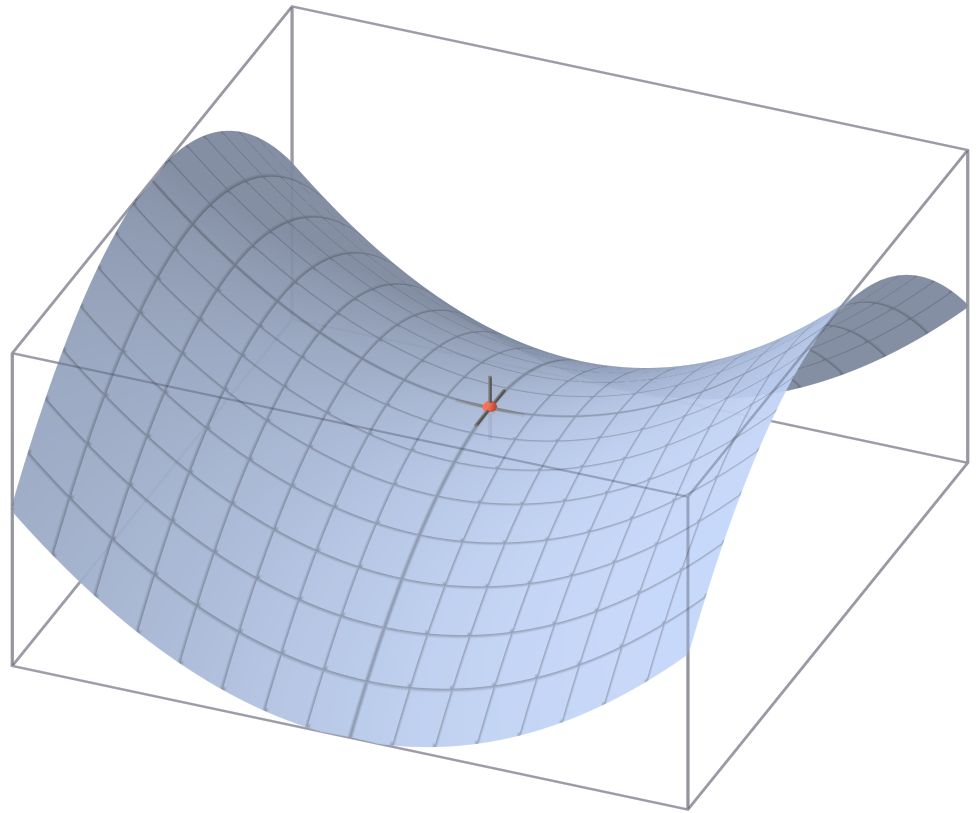
\includegraphics[width=10cm]{8_appendix/img/Saddle_point}
            \caption{Example of a saddle point.}
        \end{center}
    \end{figure}
    
    鞍点の他にも勾配がほとんど得られず学習が停滞する悪条件があり,これはプラトーと呼ばれる.
    プラトーでは損失関数の解空間が非常に平坦になるため,勾配がほとんど得られない.
    
    逆に,勾配が非常に急激な崖となっている場合も存在し,この崖の部分で損失関数は非常に大きな勾配を得る.
    すると,崖の逆方向に大きくパラメータが更新されてしまい,適切な学習が行われない場合がある.
    \begin{figure}[ht]
        \begin{center}
            \centering
            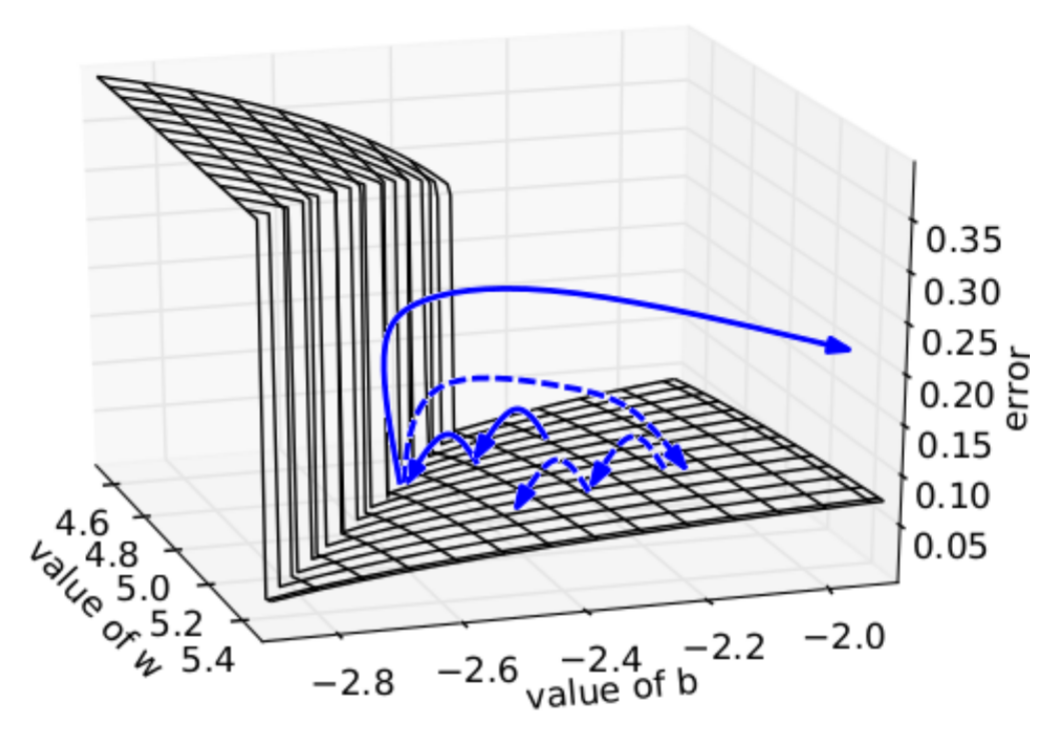
\includegraphics[width=10cm]{8_appendix/img/cliff}
            \caption{Approaching the cliff of the loss function, the slope increases and the parameters are heavily updated in the opposite direction\cite{pascanu2013difficulty}.}
        \end{center}
    \end{figure}
    しかし,この崖による勾配の爆発に関しては,勾配クリッピング\cite{pascanu2013difficulty}を行うことにより回避が可能である.

    \subsubsection{データの前処理}
    データの前処理は機械学習において非常に重要であるとされている.
    これは損失関数の解空間を考えることにより容易に理解できる.
    モデルのパラメータのスケールは,入力されるデータのスケールと線形の関係にある.
    つまり,特定のデータのスケールが他のデータのスケールと大きく異なる場合,図\ref{locc_func_scale}のように損失関数の解空間は非常に歪んだ形状になる.
    \begin{figure}[ht]
        \begin{center}
            \centering
            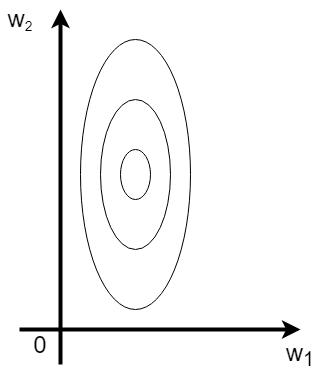
\includegraphics[width=6cm]{8_appendix/img/preprocess_lossfunc}
            \caption{A simplified diagram of how the solution space of the loss function is distorted by the scale of the parameters.}
            \label{locc_func_scale}
        \end{center}
    \end{figure}

    この損失関数で勾配を計算すると,毎回パラメータが大きく更新され,パラメータは更新のたびに大きく振動することとなり,最適化が困難になる.
    通常,機械学習で用いられるデータは$0.3<|x|<3$程度に調整されることが多い.
    このようなスケールに収めるために,以下に示すようなMin-Max Normalization(式\ref{min_max_norm})やZ-score Normalization(式\ref{z_norm})を用いてデータを正規化することが多い.
    \begin{equation}
        x_{new} = (x - x_{min}) / (x_{max} - x_{min})
        \label{min_max_norm}
    \end{equation}
    \begin{equation}
        x_{new} = (x - x_{\rm{mean}}) / x_{\rm{std}}
        \label{z_norm}
    \end{equation}

\subsection{誤差逆伝播法}
    前項において非常に複雑なニューラルネットワークを勾配によって最適化することを示した.
    線形回帰やロジスティック回帰はパラメータはたかだか一度の非線形変換を施されているだけであり,非線形変換が微分可能であれば各パラメータについて勾配を求めるのは容易である.
    しかし,ニューラルネットワークの場合には多数の非線形変換が繰り返し適用されており,個々のパラメータの勾配計算が困難である.
    この学習の困難さが長らくパーセプトロンによるニューラルネットワークの発展の障害となっていた.
    しかしその後,1986年に\cite{rumelhart1986learning}らによって誤差逆伝搬法が提案され,その問題が解決された.

    誤差逆伝搬法とは,入力$x$に対して,目標とする出力$t$と実際の$x$をニューラルネットワークに入力し,得られた出力${y}$の誤差から,ニューラルネットワークを構成するニューロンのパラメータを更新し,入力$x$に対してより目標に近い$y$が出力できるよう効率的に学習するアルゴリズムである.以下\ref{fig:neural_net_with_f}のような,入力層,隠れ層,出力層で構成された,順伝播型ニューラルネットワークが誤差逆伝搬法によってどのように学習されるか説明する.
    \begin{figure}[ht]
        \centering
        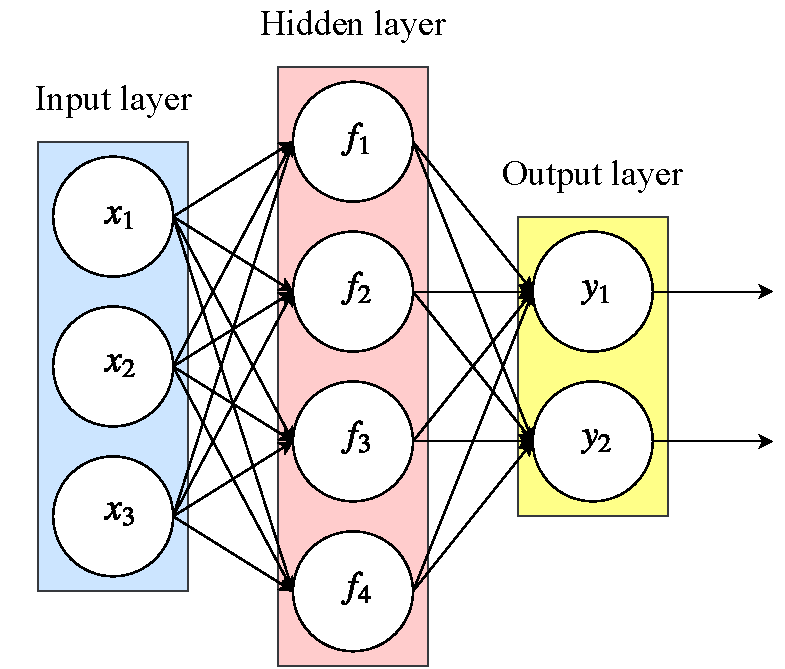
\includegraphics[width=12cm]{8_appendix/img/three_layer_nn.pdf}
        \caption{Three-layer feed-forward neural network.}
        \label{fig:neural_net_with_f}
    \end{figure}
    一方で,最終的な出力は各層の各ニューロンのネットワークの重みやバイアスによって定まるため,ニューラルネットワークの重みやバイアスといったそれぞれのパラメータをどのように更新すれば良いのか求める必要がある.
    ここで,誤差$E$はネットワーク上のすべてのパラメータに関する関数として考えられるため,ネットワークの重みやバイアスと言った学習パラメータ$p$に対して上記のニューラルネットワークの出力$\bm{y}$の更新条件と同様な条件が成り立ち,式\ref{eq:e_y_result}と同様に更新することが出来れば良い.したがって以下の式が成り立つ.
    \begin{align}
      p \to p - \eta \frac{\partial E}{\partial p}
      \label{eq:p_y_result}
    \end{align}
    このように,学習パラメータをある評価関数の勾配に基づいて更新を繰り返し,学習を行うアルゴリズムを最急降下法という.誤差逆伝搬法においては,このアルゴリズムを用いて学習行う.
    
    次に,誤差逆伝搬法において効率的に各パラメータに関する勾配を求める方法について説明する.
    全$\text{N}$層の順伝播型ニューラルネットワークについて,$n$番目の層の$m$番目のニューロンの入出力を考える.\ref{fig:n_layer_network}にネットワーク全体の概要図と,\ref{fig:n_layer_eq}に$m$番目のニューロンの入出力に注目した図を示した.ただし,$n-1$番目の層の$i$番目のニューロンと$n$番目の層の$m$番目のニューロン間の重みを$w_{n, i, m}$,$n$番目の層の$m$番目のニューロンのバイアスを$b_{n, m}$, 入力を$I_{n, m}$, 出力を$x_{n, m}$,活性化関数を$\phi _{n, m}$とした.また$n$番目の層のニューロンの総数を$N_{n}$とした.
    \begin{figure}[ht]
      \centering
      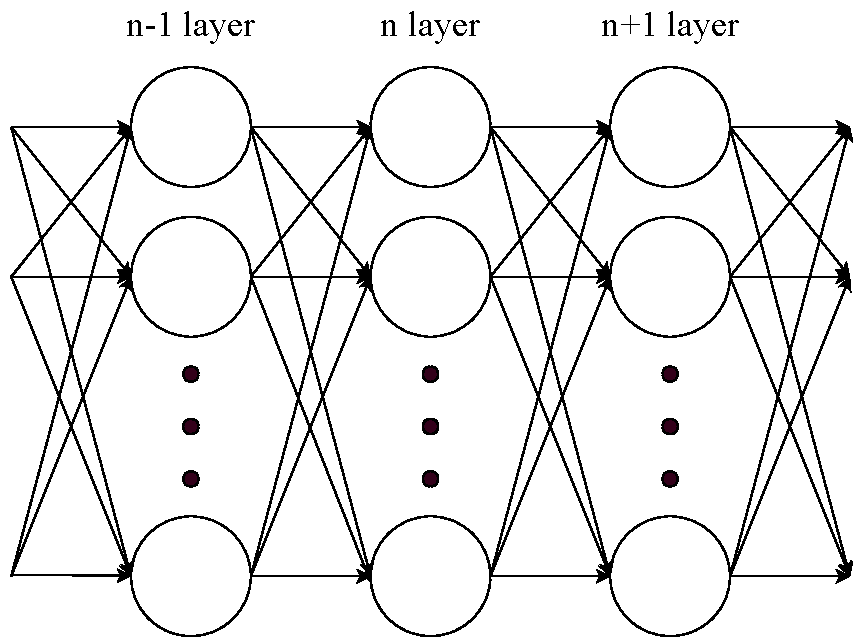
\includegraphics[width=12cm]{8_appendix/img/n_layer_network.pdf}
      \caption{N-layers neural network.}
      \label{fig:n_layer_network}
    \end{figure}
    \begin{figure}[ht]
      \centering
      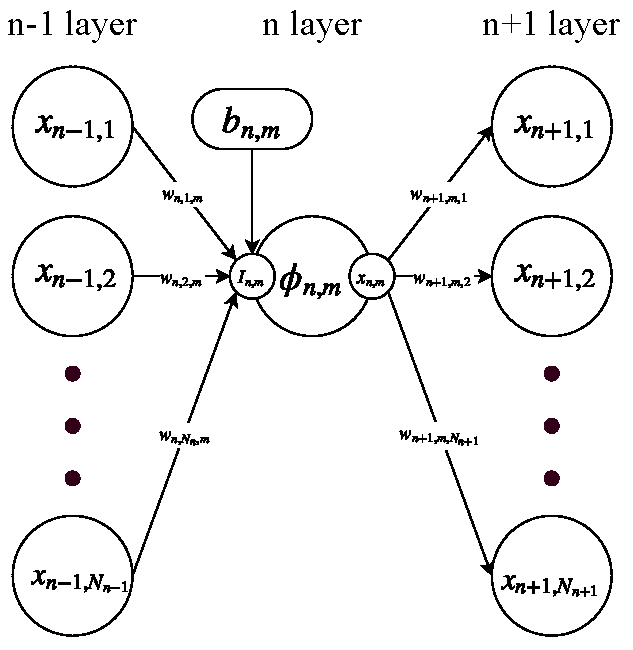
\includegraphics[width=12cm]{8_appendix/img/n_layer_eq.pdf}
      \caption{Neuron $m$ in n-layers neural network.}
      \label{fig:n_layer_eq}
    \end{figure}
    このとき,入出力関係は次式のように表される.
    \begin{align}
      I_{n, m} &= \sum_{k}^{N_{n}} w_{n, k, m} \cdot x_{n-1, k} + b_{n, m} \label{eq:i_nm} \\
      x_{n, m} &= \phi_{n, m}(I_{n, m}) \label{eq:x_nm}
    \end{align}
    次に,$n+1$層を出力層$N$としたときの,$n$層の$i$番目のニューロンと$n+1$層の$j$番目のニューロン間の重み$w_{n+1, i, j}$とバイアス$b_{n+1, j}$がどのように更新されるか求める.
    つまり,式\ref{eq:p_y_result}のように,誤差$E$を各パラメータで偏微分した値を求める.
    まず,重み$w_{n+1, i, j}$に関して,連鎖律より次式で表される.
    \begin{align}
      \frac{\partial E}{\partial w_{n+1, i, j}} &= \frac{\partial E}{\partial x_{n+1, j}} \cdot \frac{\partial x_{n+1, j}}{\partial I_{n+1, j}} \cdot \frac{\partial I_{n+1, j}}{\partial w_{n+1, i, j}}
      \label{eq:w_nim}
    \end{align}
    ここで,$\frac{\partial x_{n+1, j}}{\partial I_{n+1, j}}$,$\frac{\partial I_{n+1, j}}{\partial w_{n+1, i, j}}$は式\ref{eq:i_nm},\ref{eq:x_nm}より次式で表される.
    \begin{align}
      \frac{\partial x_{n+1, j}}{\partial I_{n+1, j}} &= \frac{\partial \phi_{n+1, j}(I_{n+1, j})}{\partial I_{n+1, j}} \nonumber \\
          &= \phi_{n+1, j}^{'}(I_{n+1, j}) \cdot (I_{n+1, j})' \nonumber \\
          &= \phi_{n+1, j}^{'}(I_{n+1, j})
          \label{eq:n_1}
    \end{align}
    \begin{align}
      \frac{\partial I_{n+1, j}}{\partial w_{n+1, i, j}} &= \frac{\partial \left( \sum_{k}^{N_{n+1}}w_{n+1, k, j}x_{n, k} + b_{n+1, j}\right)}{\partial w_{n+1, i, j}} \nonumber \\
      &= x_{n, i}
          \label{eq:n_2}
    \end{align}
    よって式\ref{eq:n_1}, \ref{eq:n_2}を式\ref{eq:w_nim}に代入すると
    \begin{align}
      \frac{\partial E}{\partial w_{n+1, i, j}} &= \frac{\partial E}{\partial x_{n+1, j}} \cdot \phi_{n+1, j}^{'}(I_{n+1, j}) \cdot x_{n, i} \label{eq:ew_n1ij}
    \end{align}
    となる.
    またバイアス$b_{n, m}$に関しても同様に計算を行うと,次式で表される.
    \begin{align}
      \frac{\partial E}{\partial b_{n+1, j}} &= \frac{\partial E}{\partial x_{n+1, j}} \cdot \phi_{n+1, j}^{'}(I_{n+1, j})
    \end{align}
    したがって,$\frac{\partial E}{\partial x_{n+1, j}}$が計算できればそれぞれのパラメータを更新することが出来る.
    
    ここで,同様の計算を$n-1$層と$n$層間でも行う.
    つまり,$n-1$層の$s$番目のニューロンと$n$層の$t$番目のニューロン間の重み$w_{n, s, t}$とバイアス$b_{n, t}$がどのように計算されるか求める.
    ここで,\ref{fig:n_layer_eq}のように,$n$層の$t$番目のニューロンが$n+1$層の$N_{n+1}$個のニューロン全てと繋がっており,これらの出力の変化に$w_{n, s, t}$が関係していることに注意し,鎖律より$ \frac{\partial E}{\partial w_{n, s, t}} $を求めると,次式のようになる.
    \begin{align}
      \frac{\partial E}{\partial w_{n, s, t}} &= \sum_{k}^{N_{n+1}}\left( \frac{\partial E}{\partial x_{n+1, k}}\cdot 
      \frac{\partial x_{n+1, k}}{\partial I_{n+1, k}}\cdot \frac{\partial I_{n+1, k}}{\partial x_{n, t}} \right)
      \cdot \frac{\partial x_{n, t}}{\partial I_{n, t}} \cdot \frac{\partial I_{n, t}}{\partial w_{n, s, t}}
      \label{eq:w_nst}
    \end{align}
    このとき,式\ref{eq:n_1}より
    \begin{align}
      \frac{\partial x_{n+1, k}}{\partial I_{n+1, k}} &= \phi _{n+1, k}(I_{n+1, k})
      \label{eq:x_n1k}
    \end{align}
    また$\frac{\partial I_{n+1, k}}{\partial x_{n, t}} $は以下の式で表される.
    \begin{align}
      \frac{\partial I_{n+1, k}}{\partial x_{n, t}} &= \frac{\sum_{i}^{N_{n+1}}w_{n+1, i, j}x_{n, i} + b_{n+1, j}}{\partial x_{n, t}} \nonumber \\
      &= w_{n+1, t, k}
      \label{eq:i_n1k}
    \end{align}
    よって,\ref{eq:w_nst}は式\ref{eq:x_n1k},\ref{eq:i_n1k}より次のようになる.
    \begin{align}
      \frac{\partial E}{\partial w_{n, s, t}} &= \sum_{k}^{N_{n+1}} \left( \frac{\partial E}{\partial x_{n+1, k}} \cdot \phi_{n+1, l}'(I_{n+1, k})\cdot w_{n+1, t, k} \right) \phi_{n, t}'(I_{n, t}) \cdot x_{n-1, s} 
    \end{align}
    ここで,$\frac{\partial E}{\partial x_{i, j}}\cdot \phi_{i, j}'(I_{i,j})$は既に$n$層と$n+1$層間でのニューロンの重みに関する式\ref{eq:ew_n1ij}にて既に計算されているため,これを$\delta_{i, j}$として整理すると次のようになる.
    \begin{align}
      \frac{\partial E}{\partial w_{n, s, t}} &= \sum_{k}^{N_{n+1}} \left( \delta_{n+1, k}\cdot w_{n+1, t, k} \right) \phi_{n, t}'(I_{n, t}) \cdot x_{n-1, s} \label{eq:ew_nst}
    \end{align}
    バイアスについても同様に次のようになる.
    \begin{align}
      \frac{\partial E}{\partial b_{n, t}} &= \sum_{k}^{N_{n+1}} \left( \delta_{n+1, k}\cdot w_{n+1, t, k} \right) \phi_{n, t}'(I_{n, t}) 
      \label{eq:eb_nt}
    \end{align}
    これらの式より,各層間での重みやバイアスといったニューラルネットワークの各パラメータを更新することで,学習することができる.
    
    また順伝播後に出力層から入力層へと順々に上記の計算を繰り返し行うことで,前層で既に求められている勾配を活用しながら各層間の各ニューロン間の重みとバイアスを更新するための勾配を求めることが出来る.
    このように,勾配を計算するための誤差が層を逆方向に伝播されて計算が行われるため,この手法は誤差逆伝搬法と呼ばれる.

    この誤差逆伝搬法によってニューラルネットワークを学習させるためには,活性化関数が微分可能である必要がある.
    そこで,パーセプトロンにおけるステップ関数を置き換えるためにシグモイド関数が活性化関数として提案された\cite{rumelhart1986learning}.
    しかし,ReLuを始めとする微分不可能な点が存在する関数は多く活性化関数として使われており,実用上は微分不可能な点が存在していても問題がないことも広く知られている.
    ただし,ステップ関数は微分値が常に0であり,誤差の逆伝播計算値が常に0となるため,誤差逆伝播を用いて最適化を行うモデルでこのような活性化関数を利用することはできない.

    また,sigmoid関数の微分値を見てみると,sigmoid関数の微分値は以下の図\ref{sigmoid_diff}のように最大値が0.25である.
    \begin{figure}[ht]
        \begin{center}
            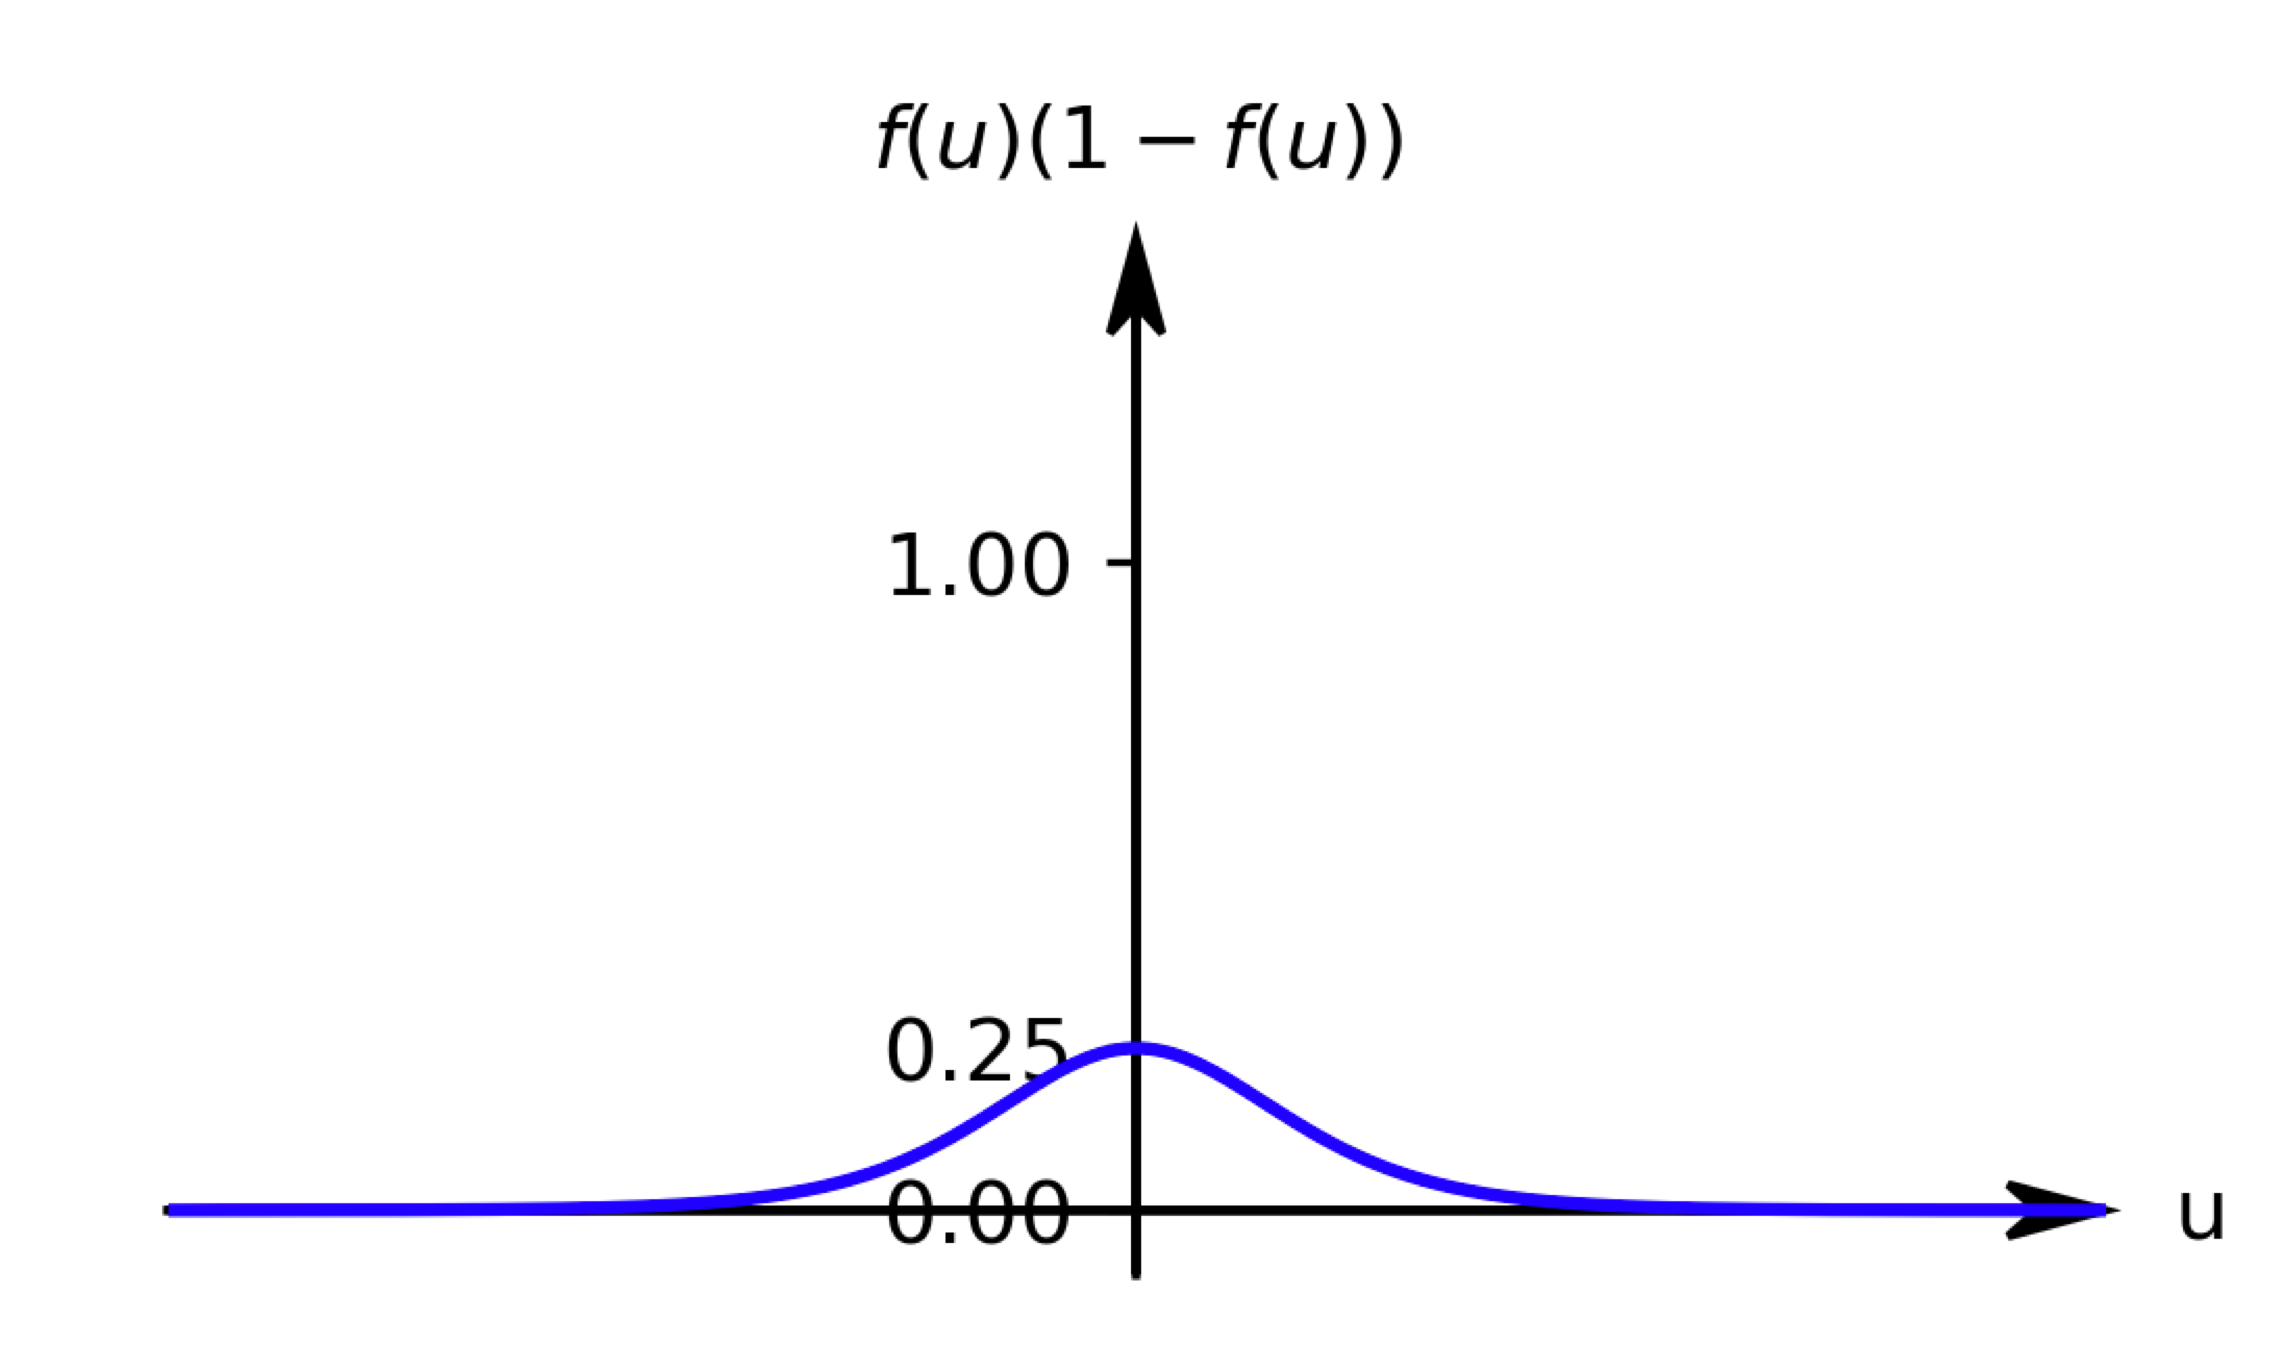
\includegraphics[width=10cm]{./8_appendix/img/sigmoid_diff.png}
            \caption{Derivatives of sigmoid functions.}
            \label{sigmoid_diff}
        \end{center}
    \end{figure}
    これは逆伝播計算の際に,繰り返しシグモイド関数が適用されるニューラルネットの浅い層になるほど,勾配の値が小さくなってしまうことを示している.
    このように浅い層になるほど勾配の値が小さくなり,深いネットワークでは浅い層に対する勾配が0付近になってしまうような現象のことを勾配消失と呼ぶ.
    これを避けるために,ニューラルネットの中間層ではReLU関数など,微分値が1に近いかそれ以上になるような活性化関数が用いられることが多い.

\subsection{様々な最適化手法}
    前項では,勾配による最適化をどのように行うかについて議論してきた.
    本項では確率的勾配降下法を改善し,勾配法の学習を最適化させる様々な手法について触れる.
    
    \subsubsection{モメンタム}
    SGDの学習をより効率的に行う方法は,大別して1次の方法および2次の方法に分類される.
    一般的にニューラルネットワークの学習では1次の方法が用いられている.
    モメンタム\cite{polyak1964some}(Momentum)は1次の方法の中でも最も一般的に使われる手法の1つで,一期前の更新量を保存することにより,更新されるパラメータの慣性を持ったような動きを実現する.
    SGDは一定の学習率を持つために学習が遅くなる傾向があるのに対し,モメンタムは学習を高速化するために設計されている.
    Momentumにおけるパラメータの更新式は以下の通りである.
    \begin{eqnarray}
        v_{t+1} &=& \alpha v_t - \eta \frac{\partial L}{\partial \theta_t}\\
        \theta_{t+1} &=& \theta_t + v_{t+1}
    \end{eqnarray}
    ここで,$\eta$は学習率を,$\alpha$はモメンタム係数を示す.($0\leq\alpha<1$)
    
    \subsubsection{Nesterov Accelerated Gradient}
    Nesterov AG\cite{mikolov2013distributed}はネステロフの加速勾配法\cite{nesterov1983method}に着想を得て開発されたモメンタムの派生系である.
    このアルゴリズムでは,一期先の位置を仮に決定し,その位置における勾配を利用することにより更新値を算出する.
    Nesterov AGにおけるパラメータの更新式を以下に示す.
    \begin{eqnarray}
        v_{t+1} &=& \alpha v_t - \eta \frac{\partial L}{\partial (\theta_t+\alpha v_t)}\\
        \theta_{t+1} &=& \theta_t + v_{t+1}
    \end{eqnarray}
    Nesterov AGを定義通りに計算するのは一期先の勾配が必要となり,計算が煩雑になる.
    したがって,現在ではBengioら\cite{bengio2013advances}が提案したアルゴリズムを採用して計算されることが多い.
    
    Nesterov AGがSGDおよびモメンタムとどのような差があるかを図\ref{SGD_update}から図\ref{Nesterov_update}で示した.
    \begin{figure}[ht]
        \begin{center}
            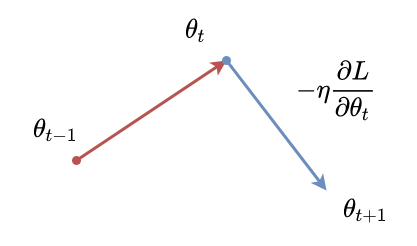
\includegraphics[width=6cm]{./8_appendix/img/SGD.png}
            \caption{Schematic diagram of parameter updates with SGD.}
            \label{SGD_update}
        \end{center}
    \end{figure}
    \begin{figure}[ht]
        \begin{center}
            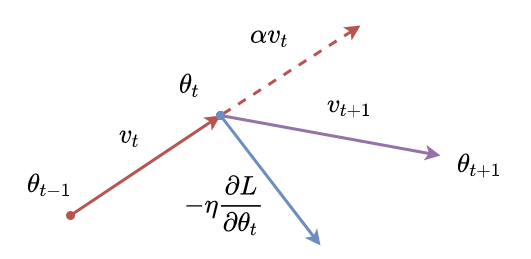
\includegraphics[width=8.5cm]{./8_appendix/img/momentum.png}
            \caption{Schematic diagram of parameter updates with Momentum.}
        \end{center}
    \end{figure}
    \begin{figure}[ht]
        \begin{center}
            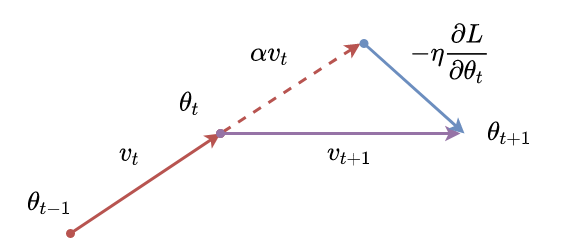
\includegraphics[width=8.5cm]{./8_appendix/img/Nesterov.png}
            \caption{Schematic diagram of parameter updates with Nesterov AG.}
            \label{Nesterov_update}
        \end{center}
    \end{figure}

    \subsubsection{AdaGrad}
    先述までの手法では学習率は任意に設定できるハイパーパラメータである上に,モデルの性能に大きな影響を与えるものであった.
    故に,学習率を損失の計算時に適応的(adaptive)に変化させる手法が多く提案されている.
    Adagrad\cite{duchi2011adaptive}はそのような適応的に学習率が変化するような手法の1つであり,学習が進むにつれ見かけの学習率が減衰していくように設計されている.
    この手法において,学習率は過去の学習率の二乗和の平方根に反比例するようにスケーリングされる.
    Adagradにおけるパラメータの更新式を以下に示す.
    \begin{eqnarray}
        \boldsymbol{h}_{t+1} &=& \boldsymbol{h}_{t}+\frac{\partial L}{\partial \boldsymbol{\theta}_{t}} \odot \frac{\partial L}{\partial \boldsymbol{\theta}_{t}} \\
        \boldsymbol{\theta}_{t+1} &=& \boldsymbol{\theta}_{t}-\eta \frac{1}{\varepsilon+\sqrt{\boldsymbol{h}_{t+1}}} \odot \frac{\partial L}{\partial \boldsymbol{\theta}_{t}}
    \end{eqnarray}
    ここで,$\varepsilon$は数値的安定性のために導入されている微小値であり,通常およそ$10^{-7}$に設定されている.
    また,$\odot$はアダマール積を表す.

    学習が進むにつれて見かけの学習率である$1/\varepsilon+\sqrt{\boldsymbol{h}_{t+1}}$が減衰することが分かる.
    しかし,AdaGradは学習は学習初期から勾配の2乗の累計を計算するために,学習率が過剰に減衰する.
    そのため,経験的にはAdaGradは常に良好な結果を残す最適化手法ではないことが知られている.
    
    \subsubsection{RMSProp}
    RMSProp\cite{hinton2012neural}は先述のAdaGradを修正し,勾配の二乗の移動平均を用いて見かけの学習率を変化させることによって,AdaGradの性能を改善させた.
    ここで,移動平均とは指数平滑化移動平均のことであり,減衰率$\rho$の割合で過去の勾配を足し合わせることにより,累積される情報は過去のものから指数関数的に減衰していく.
    RMSPropにおけるパラメータの更新式を以下に示す.
    \begin{eqnarray}
        \boldsymbol{h}_{t+1} &=& \rho \boldsymbol{h}_{t}+(1-\rho) \frac{\partial L}{\partial \boldsymbol{\theta}_{t}} \odot \frac{\partial L}{\partial \boldsymbol{\theta}_{t}} \\
        \boldsymbol{\theta}_{t+1} &=& \boldsymbol{\theta}_{t}-\eta \frac{1}{\sqrt{\varepsilon+\boldsymbol{h}_{t+1}}} \odot \frac{\partial L}{\partial \boldsymbol{\theta}_{t}}
    \end{eqnarray}
    
    \subsubsection{AdaDelta}
    AdaDelta\cite{zeiler2012adadelta}も先述のRMSPropと同様にAdaGradを修正した最適化手法の1つである.
    RMSPropが勾配の二乗の移動平均のみを用いて学習率を変化させるのに対し,AdaDeltaは勾配の二乗の移動平均に加えて,更新量の二乗の移動平均を用いて見かけの学習率を変化させる.
    AdaDeltaにおけるパラメータの更新式を以下に示す.
    \begin{eqnarray}
        \boldsymbol{h}_{t+1}&=&\rho \boldsymbol{h}_{t}+(1-\rho) \frac{\partial L}{\partial \boldsymbol{\theta}_{t}} \odot \frac{\partial L}{\partial \boldsymbol{\theta}_{t}} \\
        \Delta \boldsymbol{\theta}_{t}&=&-\frac{\sqrt{\varepsilon+\boldsymbol{r}_{t}}}{\sqrt{\varepsilon+\boldsymbol{h}_{t+1}}} \odot \frac{\partial L}{\partial \boldsymbol{\theta}_{t}} \\
        \boldsymbol{\theta}_{t+1}&=&\boldsymbol{\theta}_{t}+\Delta \boldsymbol{\theta}_{t} \\
        \boldsymbol{r}_{t+1}&=&\rho \boldsymbol{r}_{t}+(1-\rho) \Delta \boldsymbol{\theta}_{t} \odot \Delta \boldsymbol{\theta}_{t}
    \end{eqnarray}
    上記のように,更新量の二乗の移動平均を導入することにより,極小値付近でこの値が非常に小さい値になり,動きが遅くなる.
    また,学習率$\eta$が更新量の移動平均と置き換えられ,単位を揃える働きをしていることに注意されたい.
    
    \subsubsection{Adam}
    Adam\cite{kingma2014adam}はRMSpropおよびモメンタムを同時に適用したような手法であり,学習率の変化にも頑健で,現在最も良く利用されている最適化手法の1つに数えられる.
    AdamとRMSpropおよびモメンタムには若干の差が存在する.
    Goodfellowら\cite{Goodfellow-et-al-2016}は以下の2つの差異を指摘している.
    1つ目は,モメンタムをRMSpropに追加する最も単純な方法は,再スケーリングされた勾配にモメンタムを適用することだが,Adamでは式\ref{adam_momentum}のように,1次モーメントが直接導入されていることである.
    そして,2つ目は1次モーメントおよび2次モーメント両方の推定へのバイアス補正が含まれており,原点での初期化が考慮されていない点である.
    
    \begin{eqnarray}
        \boldsymbol{m}_{t+1} &=&\rho_{1} \boldsymbol{m}_{t}+\left(1-\rho_{1}\right) \frac{\partial L}{\partial \boldsymbol{\theta}_{t}} \label{adam_momentum}\\
        \boldsymbol{v}_{t+1} &=&\rho_{2} \boldsymbol{v}_{t}+\left(1-\rho_{2}\right) \frac{\partial L}{\partial \boldsymbol{\theta}_{t}} \odot \frac{\partial L}{\partial \boldsymbol{\theta}_{t}} \\
        \widehat{\boldsymbol{m}}_{t+1} &=&\frac{\boldsymbol{m}_{t+1}}{1-\rho_{1}^{t}} \\
        \widehat{\boldsymbol{v}}_{t+1} &=&\frac{\boldsymbol{v}_{t+1}}{1-\rho_{2}^{t}} \\
        \boldsymbol{\theta}_{t+1} &=&\boldsymbol{\theta}_{t}-\eta \frac{1}{\sqrt{\hat{\boldsymbol{v}}_{t+1}}+\varepsilon} \odot \widehat{\boldsymbol{m}}_{t+1}
    \end{eqnarray}

\subsection{深層学習における正則化}
    過学習はニューラルネットワークの学習においても発生する.
    過学習は訓練誤差に比べ汎化誤差が大きくなる現象であり,パラメータが多い場合や,訓練データの数が少ない場合などに発生しやすい.
    その意味で言えばニューラルネットワークは膨大なパラメータを有しているために,過学習が非常に起きやすい.
    この過学習に対応するために,パラメータに制限を設けるなどの対応が行われ,これは正則化と呼ばれている.
    本節では,前節で触れたL2正則化に触れつつ,ニューラルネットワークの訓練における正則化手法を複数示す.

    \subsubsection{荷重減衰}
    荷重減衰(weight decay)は最も一般的な正則化手法の1つであり,重みの値が大きくなることにペナルティを与えることによって過学習を抑制している.
    荷重減衰では,損失関数の全ての層に$1/2\lambda w_{ij}^2$を加える.
    これは前節で触れたL2正則化と同様であり,この項をL2ノルムと呼ぶ.
    ここで$\lambda$は通常$1.0^{-2}$~$1.0^{-5}$程度の値が利用されることが多い.
    また,ニューラルネットワークにおける荷重減衰は,アフィン変換の重みにのみ適用され,通常バイアス項には適用されないことに注意されたい.

    \subsubsection{早期終了}
    早期終了(early stoppting)は,一定のルールを満たした場合に学習を終了させる手法であり,一般に過学習抑制効果がある\cite{bishop1995regularization,sjoberg1995overtraining}.
    早期終了の学習終了基準は非常に単純である.
    学習の各ステップにおけるテスト用データの検証誤差(validation loss)を算出し,前ステップの検証誤差と比較する.
    現ステップの検証誤差が前ステップよりも高かった場合カウンタに1を加算し,このカウンタが指定回数以上になった場合に学習を終了させる.
    ここでの指定回数はハイパーパラメータとなる.
    
    \subsubsection{ドロップアウト}
    ドロップアウト\cite{srivastava2014dropout}(dropout)は,ノードをランダムに消去しながら学習する方法であり,過学習を抑制する効果がある.
    過学習抑制に有効な手法としてアンサンブル学習があり,アンサンブル学習の中でも複数のモデルを組み合わせて予測を頑健にする手法をバギングと呼ぶ.
    バギングは非常に計算コストが高く実用的でない場合が多い.
    ドロップアウトは,複数のネットワークをアンサンブル学習していると解釈できることから,バギングの近似であると表現されることがある.
    
    ドロップアウトの発想は比較的簡単である.
    各ミニバッチに対して,消去するノードを確率$p$でランダムに選択し,順伝播計算および逆伝播計算を行う.
    このとき,消去したノードは順伝播および逆伝播のどちらでも使うことはない.
    そして,予測時には全てのノードを採用する.このとき,全ての重みに$(1-p)$を一律で掛け合わせる.
    この操作は全てのノードを採用することによって,学習時に比べて出力値が大きくなることを是正している.
    \begin{figure}[ht]
        \begin{center}
            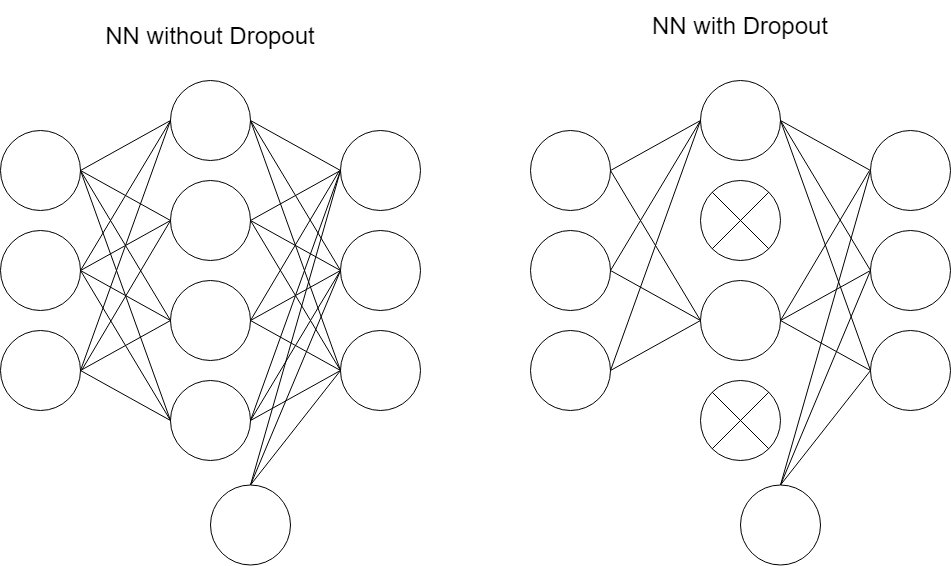
\includegraphics[width=12cm]{./8_appendix/img/dropout.png}
            \caption{Dropout}
        \end{center}
    \end{figure}

    ドロップアウトは特に全結合層に対してのみ適用されることが多く,畳込み層に適用される機会は少ない.
  原著論文\cite{srivastava2014dropout}では畳み込み層が持つパラメータが少ないため、ドロップアウトが持つ正則化の効果が薄くなることを指摘している。
    
    \subsubsection{バッチ正規化}
    バッチ正規化\cite{ioffe2015batch}(batch normalization)とは各層のアクティベーション分布を適度な広がりを持つように調整する手法であり,活性化関数の手前に設置されることが多い.
    バッチ正規化により,学習の進行が速くなることが期待でき,ネットワークの初期値に依らない学習が可能になる.
    バッチ正規化は本来,内部共変量シフトの解決を目的に設計されたが,結果的に正則化の効果を得られることが多い.
    内部共変量シフトとは,ニューラルネットワークにおいて発生する共変量シフトのことである.
    共変量とはモデルに入力されるデータのことであり,この入力に対する出力の生成規則は訓練時とテスト時で変わらないが,入力 (共変量) の分布が訓練時とテスト時で異なるという状況のことを変量シフトと呼ぶ.
    例えば,ニューラルネットワークではステップごとにパラメータが更新され,n層目の出力(n+1層目の入力)の分布は重みが更新されるたびに変化する.
    バッチ正規化を用いることで,この共変量シフトへの対応を,一層前のパラメータ全体から,バッチ正規化の持つパラメータのみに絞ることができ,効率的な学習が可能となる.
    
    バッチ正規化の計算手順は,仮に計算対象を式\ref{cal_x}のように定めると式\ref{standlization}のように計算できる.
    \begin{equation}
        \bm{x} = \{x_1,x_2, ... ,x_n\}
        \label{cal_x}
    \end{equation}
    \begin{equation}
        y_i = \gamma \frac{x_i-\mu}{\sqrt{\sigma^2+\epsilon}} + \beta
        \label{standlization}
    \end{equation}
    
    ここで,$\beta,\gamma$は標準化された$x$の分布を最適な分布に変換するための係数であり,学習の過程で最適化されていくパラメータである.
    ここで,データの平均値および分散を表す$\mu,\sigma^2$について,予測時には学習時の移動平均を用いることに注意されたい.
    
    バッチ正規化は、現在ほとんどのモデルで導入されている。
    また、特にバッチ正規化はドロップアウトと併用されることはない。
    特に、バッチ正規化の直後にドロップアウトを使用することにより、バッチ正規化によって得られた統計的性質が阻害されるために、精度の悪化などの悪影響が報告されている\cite{li2019understanding} 。
    
    また、バッチ正規化は基本的に荷重減衰と併用することはあまり意味がないとされている。
    これは、バッチ正規化が出力スケールを入力によらず不変にするためである。
    バッチ正規化に入力される値のスケールはレイヤの重みのスケールと線形関係にある。
    バッチ正規化の出力スケールが入力によらず不変になるのであれば、モデルの重みを制限することによりレイヤーの異常な出力を抑制している荷重減衰を適用するかどうかに関わらず、バッチ正規化の出力スケールは不変であり、荷重減衰を適用する利点は薄い。
    しかし、荷重減衰を適用することにより学習率が過剰に低下するのを防止する効果も見られることから、この観点で荷重減衰を利用することは考えられる。
    この議論は様々な論文で指摘されている\cite{van2017l2, hoffer2018norm}。

    また,バッチ正規化の他にも,類似の手法がいくつか提案されている.
    例えば,レイヤー正規化\cite{ba2016layer}では,バッチ方向ではなく,レイヤーの内部のみで各データについて正規化を行っている.
    また,インスタンス正規化\cite{ulyanov2016instance}では,さらに画像内のチャンネルにのみ注目した正規化を行っている.
    これは,1チャンネル分の画像で正規化することにより,画像のコントラストを取り除くことを意図している.
    そして,グループ正規化\cite{wu2018group}では,インスタンス正規化のようにチャンネルに注目し,そのチャンネルを複数のグループにまとめてから正規化を行っている.
    これは,バッチサイズを小さくするとバッチごとの統計量の推定精度が劣化することに注目して,バッチサイズの影響を受けないような設計になっている.
    \begin{figure}[ht]
        \begin{center}
            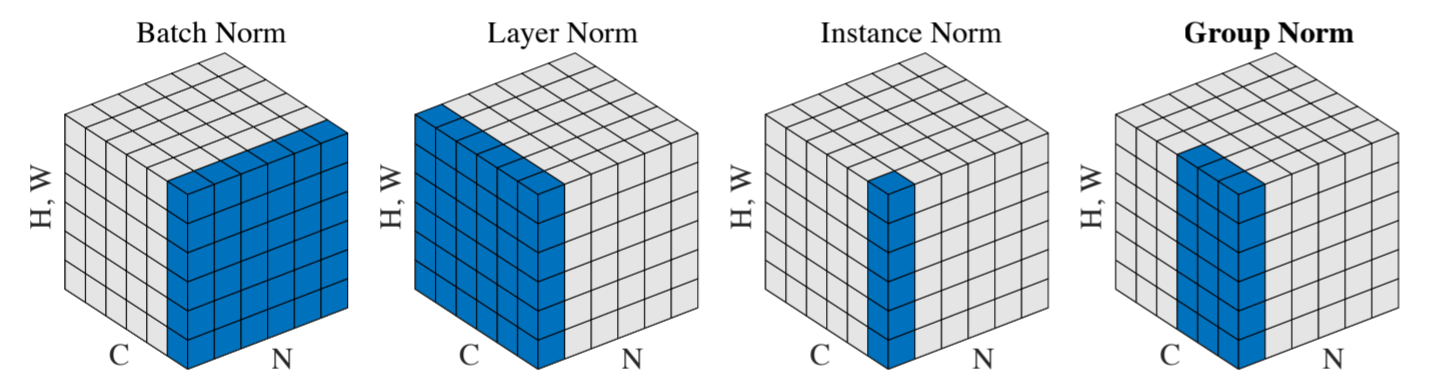
\includegraphics[width=15cm]{./8_appendix/img/batchnorm_description}
            \caption{A brief description of each normalization method\cite{wu2018group}.}
        \end{center}
    \end{figure}
